\documentclass[11pt]{exam}
\RequirePackage{amssymb, amsfonts, amsmath, latexsym, verbatim, xspace, setspace}
\RequirePackage{tikz, pgflibraryplotmarks}

\usepackage[margin=1in]{geometry}
\usepackage[utf8]{inputenc}


% Here's where you edit the Class, Exam, Date, etc.
\newcommand{\class}{Seminario de tecnología}
\newcommand{\examnum}{Examen Parcial 3}
\newcommand{\term}{2 Cuatrimestre, 2014}
\newcommand{\examdate}{14/11/14}
\newcommand{\timelimit}{120 minutos}

% For an exam, single spacing is most appropriate
\singlespacing
% \onehalfspacing
% \doublespacing

% For an exam, we generally want to turn off paragraph indentation
\parindent 0ex

\begin{document} 

% These commands set up the running header on the top of the exam pages
\pagestyle{head}
\firstpageheader{}{}{}
\runningheader{\class}{\examnum\ - Pagina \thepage\ de \numpages}{\examdate}
\runningheadrule

\begin{flushright}
\begin{tabular}{p{2.8in} r l}
\textbf{\class} & \textbf{Nombre:} & \makebox[2in]{\hrulefill}\\
\textbf{\term} &&\\
\textbf{\examnum} &&\\
\textbf{\examdate} &&\\
\textbf{Tiempo: \timelimit}
\end{tabular}\\
\end{flushright}
\rule[1ex]{\textwidth}{.1pt}

\begin{minipage}[t]{3.7in}
Este examen consta de \numpages\ paginas y \numquestions\ preguntas. Verifique que tiene todas las hojas necesarias. Las preguntas se responden en la misma hoja del examen.\\

El examen se puede realizar a libro abierto y esta permitido el uso de calculadora si es requerido. Se puede utilizar computadora.\\

Las siguientes reglas aplican para la aprobación del examen:\\
\vspace{0pt}
\begin{itemize}
\item Escritura de todas las \textbf{respuestas en tinta, sin excepción}.-
\item \textbf{Se requiere un mínimo de 10 puntos} para la aprobación del examen.-
\item Justificar sus respuestas, en caso de ser necesario, con diagramas o ejemplos claro.-
\item Lea todo el examen antes de comenzar a responder. Algunas preguntas guardan relación con otras y pueden servir de ayuda.-
\end{itemize}

No escriba en la tabla de la derecha.\\
\\
\textbf{Mucha suerte! :)}

\end{minipage}
\hfill
\begin{minipage}[t]{2.3in}
\vspace{0pt}
%\cellwidth{3em}
\gradetablestretch{2}
\vqword{Pregunta}
\addpoints % required here by exam.cls, even though questions haven't started yet.	
\gradetable[v]%[pages]  % Use [pages] to have grading table by page instead of question

\end{minipage}
\newpage % End of cover page

%%%%%%%%%%%%%%%%%%%%%%%%%%%%%%%%%%%%%%%%%%%%%%%%%%%%%%%%%%%%%%%%%%%%%%%%%%%%%%%%%%%%%
%
% See http://www-math.mit.edu/~psh/#ExamCls for full documentation, but the questions
% below give an idea of how to write questions [with parts] and have the points
% tracked automatically on the cover page.
%
%
%%%%%%%%%%%%%%%%%%%%%%%%%%%%%%%%%%%%%%%%%%%%%%%%%%%%%%%%%%%%%%%%%%%%%%%%%%%%%%%%%%%%%

\begin{questions}

% Pregunta 1
\addpoints
\question[2] Defina el concepto de Minería de datos.
\vspace{3in}

% Pregunta 2
\addpoints
\question[2] Defina el concepto de cluster de datos. A que se refiere el concepto de clusterización?
\vspace{3in}

% Pregunta 3
\addpoints
\question[1] Indique cual/es de las siguientes herramientas se utilizan para análisis estadístico de clusters:
\begin{itemize}
\item SPSS
\item Weka
\item Qucs
\end{itemize}

\newpage
% Pregunta 4
\addpoints
\question[2] \textbf{Indicar verdadero o falso}. Se desea crear un modelo regresión lineal a partir de un data set de entrenamiento. Agregar variables al modelo original siempre reducirá la suma de los cuadrados residuales medidos en el set de validación? \textbf{Justificar}.
\vspace{1in}

% Pregunta 5
\addpoints
\question[1] \textbf{Indicar verdadero o falso}. Aunque la selección hacia adelante (forward) y la eliminación hacia atrás (backward) son métodos rápidos para la selección de subconjuntos en regresión lineal, solo la selección por etapas garantiza encontrar el mejor subconjunto. \textbf{Justificar}.
\vspace{1in}

% Pregunta 6
\addpoints
\question[1] \textbf{Indicar verdadero o falso}. Un grupo de funciones de clasificación se ordenan utilizando el análisis discriminante para un conjunto de datos con tres clases $C1$, $C2$ y $C3$. Se asume que las tres clases son igualmente propensas a surgir en la aplicación. Posteriormente, se conoce que la probabilidad de $C1$ es el doble que la de $C2$ y $C3$. Las probabilidades para $C2$ y $C3$ son iguales. Si se  vuelven a calcular las funciones de clasificación utilizando esta información, el valor de la función de clasificación para $C1$ se incrementará para cada punto de datos. \textbf{Justificar}.
\vspace{1in}

% Pregunta 7
\addpoints
\question[1] \textbf{Indicar verdadero o falso}. La tasa de errores de clasificación de un modelo de clasificación en el conjunto de validación es la mejor medida de la capacidad predictiva del modelo en los nuevos datos, a diferencia de su tasa de errores de clasificación en el conjunto de entrenamiento. \textbf{Justificar}.
\vspace{1in}

% Pregunta 8
\addpoints
\question[1] \textbf{Indicar verdadero o falso}. Un clasificador de redes neuronales para dos clases construye un límite de separación entre las clases que es lineal en sumas ponderadas de los valores de entrada. \textbf{Justificar}.

\newpage
% Pregunta 9
\addpoints
\question[1] Un conjunto de datos de 1.000 casos fue dividido en un conjunto de entrenamiento de 600 casos y un conjunto de validación de 400 casos. Un \textbf{k-Nearest Neighbors} con k = 1 tiene una tasa de error de clasificación del 8\% sobre los datos de validación. Posteriormente se descubrió que la división se había hecho de forma incorrecta y que 100 casos del conjunto de datos de entrenamiento se había duplicado y accidentalmente había sobreescrito 100 casos en el conjunto de datos de validación. ¿Cuál es la tasa de error de clasificación para los 300 casos que estaban verdaderamente parte de la validación de datos?
\vspace{2in}

% Pregunta 10
\addpoints
\question[2] Describa las etapas del proceso de generación de un modelo de minería de datos.
%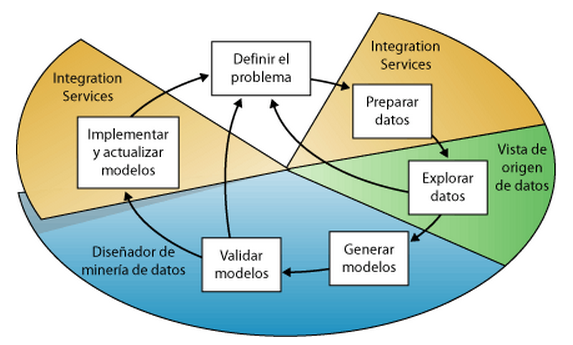
\includegraphics[scale=0.35]{steps}
\vspace{2in}


% Pregunta 11
\addpoints
\question[1] \textbf{Indique la opcion correcta.} El modelo de minería de datos que crea un algoritmo a partir de los datos puede tomar diversas formas, incluyendo:

\begin{enumerate}
\item Un conjunto de clústeres que describe cómo se relacionan los casos de un conjunto de datos.
\item Un árbol de decisión que predice un resultado y que describe cómo afectan a este los distintos criterios.
\item Un modelo matemático que predice las ventas.
\item Un conjunto de reglas que describen cómo se agrupan los productos en una transacción, y las probabilidades de que dichos productos se adquieran juntos.
\item Ninguno de los anteriores
\item Los itemas 1, 2, 3 y 4.
\end{enumerate}


\newpage
% Pregunta 12
\addpoints
\question[2] Los algoritmos para el analisis de datos se pueden elegir, entre otros cosas, segun el tipo de analisis que se quiere realizar. Describa esta clasificacion.
\vspace{3in}

% Pregunta 13
\addpoints
\question[1] \textbf{Indique la opcion correcta.} La configuración de una estructura de minería de datos consta de 5 pasos. Marque cual de ellos es opcional.

\begin{itemize}
\item Definir un origen de datos.
\item Seleccionar las columnas de datos que se van a incluir en la estructura (no es necesario agregar todas las columnas al modelo) y definir una clave.
\item Definir una clave para la estructura, incluyendo la clave de la tabla anidada, si procede.
\item Especificar si los datos de origen se deben separar en un conjunto de entrenamiento y en un conjunto de prueba.
\item Procesar la estructura.
\end{itemize}

% Pregunta 14
\addpoints
\question[1] Defina el concepto de outlier. Porque es importante preprocesar la informacion y encontrar este tipo de datos?
\vspace{1in}

% Pregunta 15
\addpoints
\question[1] Existen 3 (tres) criterios para validar los modelos de minería de datos. Cuales son? Describalos.
\vspace{4.5in}
\end{questions}
\end{document}